\documentclass[tikz]{standalone}

\definecolor{n0}{HTML}{785EF0}
\definecolor{End}{HTML}{DC267F}
\definecolor{Corner}{HTML}{FFB000}
\definecolor{NewHex}{HTML}{648FFF}
\definecolor{Reversal}{HTML}{FE6100}

\begin{document}
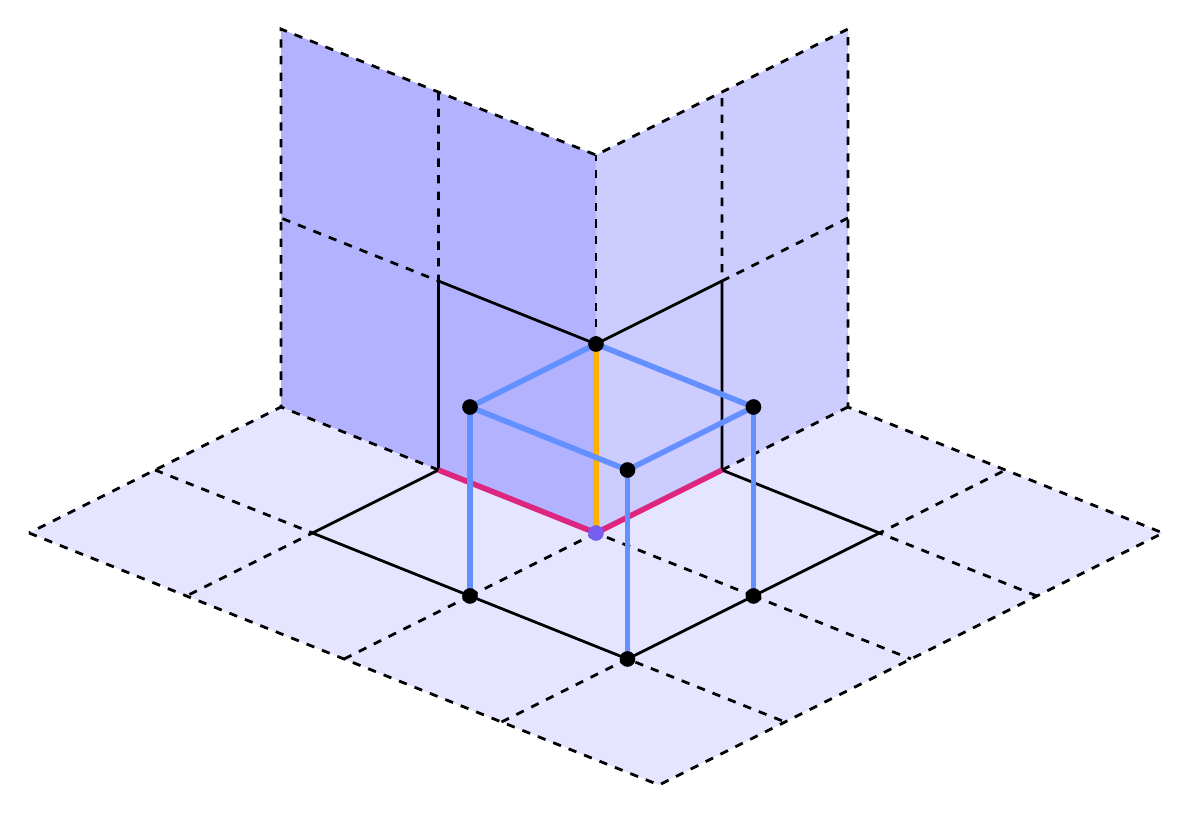
\begin{tikzpicture}[scale=4, x={(0.5cm,-0.2cm)}, y={(0.4cm,0.2cm)}, z={(0.0cm,0.6cm)}]

  %%%%%%%%%% Points pour travailler %%%%%%%%%%

 \coordinate (0) at (0,1,0);
 \coordinate (1) at (0,2,0);
 \coordinate (2) at (1,0,0);
 \coordinate (3) at (1,1,0);
 \coordinate (4) at (1,2,0);
 \coordinate (5) at (2,0,0);
 \coordinate (6) at (2,1,0);
 \coordinate (7) at (2,2,0);
 \coordinate (8) at (2,3,0);
 \coordinate (9) at (2,4,0);
 \coordinate (10) at (3,0,0);
 \coordinate (11) at (3,1,0);
 \coordinate (12) at (3,2,0);
 \coordinate (13) at (3,3,0);
 \coordinate (14) at (3,4,0);
 \coordinate (15) at (4,1,0);
 \coordinate (16) at (4,2,0);
 \coordinate (17) at (4,3,0);
 \coordinate (18) at (0,2,1);
 \coordinate (19) at (1,2,1);
 \coordinate (20) at (2,1,1);
 \coordinate (21) at (2,2,1);
 \coordinate (22) at (2,3,1);
 \coordinate (23) at (2,4,1);
 \coordinate (24) at (3,1,1);
 \coordinate (25) at (3,2,1);
 \coordinate (26) at (1,2,2);
 \coordinate (27) at (2,2,2);
 \coordinate (28) at (2,3,2);

 \coordinate (29) at (0,0,0);
 \coordinate (30) at (4,0,0);
 \coordinate (31) at (4,4,0);
 \coordinate (32) at (2,4,2);
 \coordinate (33) at (0,2,2);

 
 %%%%%%%%%% Layer blue color %%%%%%%%%%
 \fill [color=blue!30!white] (7) -- (1) -- (33) -- (27) -- cycle ;
 \fill [color=blue!20!white] (7) -- (9) -- (32) -- (27) -- cycle ;
 \fill [color=blue!10!white] (1) -- (7) -- (9) -- (31) -- (30) -- (29) -- cycle ;
 
 % Precedant layer
 \draw [line width=1] (3) -- (11) ;
 \draw [line width=1] (11) -- (13) ;
 \draw [line width=1] (7) -- (21) ;

 \draw [line width=1] (3) -- (4) -- (19) ;
 \draw [line width=1] (13) -- (8) -- (22) ;
 \draw [line width=1] (19) -- (21) -- (22) ;

 \draw [dashed, line width=1] (0) -- (3) -- (2) ;
 \draw [dashed, line width=1] (5) -- (6) ;
 \draw [dashed, line width=1] (10) -- (11) -- (15) ;
 \draw [dashed, line width=1] (12) -- (16) ;
 \draw [dashed, line width=1] (17) -- (13) -- (14) ;
 \draw [dashed, line width=1] (8) -- (9) ;
 \draw [dashed, line width=1] (23) -- (22) -- (28) ;
 \draw [dashed, line width=1] (21) -- (27) ;
 \draw [dashed, line width=1] (26) -- (19) -- (18) ;
 \draw [dashed, line width=1] (4) -- (1) ;
 \draw [dashed, line width=1] (29) -- (30) -- (31) -- (9) -- (32) -- (27) -- (33) -- (1) -- (29) ;
 
 
 %%%%%%%%%%% Feature edges %%%%%%%%%%%
 \draw [line width=2, color=End] (7) -- (4) ;
 \draw [line width=2, color=End] (7) -- (8) ;
 \draw [line width=2, color=Corner] (7) -- (21) ;
 
 %%%%%%%%%%% The HEXA created %%%%%%%%%%%
 %\draw [line width=2, color=black] (6) -- (11) -- (12) ;
 \draw [dashed, line width=1, color=black] (6) -- (7) ;
 \draw [dashed, line width=1, color=black] (12) -- (7) ;
 
 \draw [line width=2, color=NewHex] (20) -- (21) -- (25) -- (24) -- (20) ;
 \draw [line width=2, color=NewHex] (6) -- (20) ;
 \draw [line width=2, color=NewHex] (11) -- (24) ;
 \draw [line width=2, color=NewHex] (12) -- (25) ;

  %%%%%%%%%%% HEXA NODES %%%%%%%%%%%
 \draw (7) node[circle, fill=n0, inner sep = 2 pt] {};
 \draw (6) node[circle, fill=black, inner sep = 2 pt] {};
 \draw (11) node[circle, fill=black, inner sep = 2 pt] {};
 \draw (12) node[circle, fill=black, inner sep = 2 pt] {};
 \draw (20) node[circle, fill=black, inner sep = 2 pt] {};
 \draw (21) node[circle, fill=black, inner sep = 2 pt] {};
 \draw (24) node[circle, fill=black, inner sep = 2 pt] {};
 \draw (25) node[circle, fill=black, inner sep = 2 pt] {};

\end{tikzpicture}
\end{document}